\documentclass[fleqn,10pt]{wlscirep}
\usepackage[T1]{fontenc}
\usepackage{lineno}
\linenumbers
% \documentclass[a4paper,10pt]{article}
\usepackage[utf8]{inputenc}
\usepackage{authblk}
\usepackage{tabularx}
\usepackage{url}
\usepackage{graphicx}
\graphicspath{{images/}}
\usepackage{caption}
\usepackage{subcaption}
\usepackage{multirow}
\usepackage{multicol}
\usepackage{listings}
\usepackage{placeins}

\title{SuperMat: Construction of a linked annotated dataset from superconductors-related publications}

\author[1]{Luca Foppiano}
\author[1]{Sae Dieb}
\author[1]{Akira Suzuki}
\author[2]{Pedro Baptista de Castro}
\author[2]{Suguru Iwasaki}
\author[2]{Azusa Uzuki}
\author[2]{Miren Garbine Esparza Echevarria}
\author[2]{Yan Meng}
\author[2]{Kensei Terashima}
\author[3]{Laurent Romary}
\author[2]{Yoshihiko Takano}
\author[1*]{Masashi Ishii}

\affil[1]{Material Database Group, MaDIS, NIMS, Tsukuba, 305-0044, Japan}
\affil[2]{Nano Frontier Superconducting Materials Group, MANA, NIMS, Tsukuba, 305-0047, Japan}
\affil[3]{ALMAnaCH, Inria, Paris, 75012, France}

\affil[*]{corresponding author(s): Masashi Ishii (ISHII.Masashi@nims.go.jp)}


\begin{abstract}
In superconducting materials science, abundant publications are available as knowledge sources, although not suitable as a machine-readable source.
Thus, the development of text and data mining (TDM) processes is necessary to exploit such prosperity of information by providing efficient access to this accumulated knowledge, paving the way for use in data-driven superconducting materials design. 
In this paper, we present SuperMat (Superconductor Materials), an annotated corpus of linked data from superconductors scientific publications. The corpus is Composed of 145 articles and 9966 entities [TODO: update figures], annotated for six categories including names, classes and properties of materials, and the links to their respective superconducting critical temperature (\textit{T\textsubscript{c}}) and parametric conditions such as applied pressure or measurement methods.
The construction of SuperMat is the result of a fruitful collaboration between computers- and material- scientists, ensuring sound quality through  the validation from domain-experts. 
The consistency and the quality of the annotations guidelines are ensured by obtaining a satisfying Inter Annotator Agreement (IAA) between annotators and domain-experts. 
SuperMat includes the dataset, the annotation guidelines and the annotation support tools with the use of automatic annotations suggestions that help minimising the human annotation errors.
\end{abstract}

\begin{document}
\flushbottom
\maketitle

\section*{Background and summary}
The vast majority of scientific knowledge is available with overwhelming abundance~\cite{Grigas2017JustGI, Khabsa2014TheNO, OrduaMalea2015MethodsFE, Bjrk2009ScientificJP} through published papers and articles. 
However, most of the information is presented as text, which is an arbitrary and unstructured form of communication that is challenging to be used as machine-readable media. 
The computer-assisted process for collecting information from scientific literature, which is part of the text and data mining (TDM) discipline, is a supportive asset for scientific research. 
In the past decades, TDM processes have evolved their ability to perform automatic document processing such as information retrieval, entity extraction, and clustering, in several natural sciences.  

For example, in biology, TDM has been applied in information extraction to identify agents interaction (e.g. bacteria, virus, genes, proteins)~\cite{10.1371/journal.pone.0004554, Krallinger2010, Krallinger2009ExtractionOH} or to support the research against serious diseases, like cancer~\cite{Krasnitz2019CancerB}. 
Chemical compounds name disambiguation, synthesis extraction and retrieval, are other applications in chemistry~\cite{Hawizy2011ChemicalTaggerAT}.
In both domains, such applications were based on manually curated datasets (corpora) as infrastructures for their TDM systems-for example, BioCreative IV CHEMDNER corpus~\cite{Krallinger2015TheCC} in chemistry, and Genia~\cite{Kim2003GENIAC} and GENETAG~\cite{Tanabe2005GENETAGAT, Ohta2009IncorporatingGA} in biology. The availability of such datasets is a crucial requirement for developing, training, and evaluating TDM systems.

In the materials science domain, however, there are only limited resources. We can mention NaDev~\cite{Dieb2016} to support the research of nanocrystal devices and, a material-synthesis corpus, for extracting synthesis recipes~\cite{kononova_text-mined_2019}. 
To cover this shortage of infrastructure, ab-initio calculations are sometimes used~\cite{Jain2013CommentaryTM_materialsProject} but they do not necessarily describe the real system. While, most of the available experimental datasets were extracted manually~\cite{doi:10.1021/cm400893e}. 
Moreover, there are several difficulties for enabling data-driven material exploration (also called Materials Informatics (MI)): lack of data standard, infancy of the data-driven culture, wide variety of conflicting stack-holders, and missing incentives to contribute to large collaborative initiatives~\cite{Hill2016MaterialsSW}. 
It is necessary to fill this gap by creating infrastructural resources to support TDM processes in materials science based on automatic construction of databases for materials and their properties. 
Such application can save the cost of manually reading the new papers to extract the reported materials and their properties. 
Additionally, and equally important, it enables scientists to focus and leverage computing power and human resources for finding deeper relationships between information potentially unrelated. 
Other examples include providing semantically enriched search engines accepting fine-grain queries~\cite{Liu2019SurfaceMR} to reduce the time needed to access specific information. 
All these processes cannot be established without essential resources like dictionaries, lexicons, and datasets. 

% Superconductors domain
Superconducting materials research is among many fields in materials research where materials superconductivity is being studied for both fundamental and applications. It is characterised by intriguing phenomena such as zero-resistivity, ability to host high magnetic field, quantisation of the magnetic flux, and vortex pinning.  
There are many superconductor applications currently in use from daily-life to fundamental research, such as medical instruments, high-speed trains, quantum computers, and the Linear Hadron Collider (LHC)~\cite{PhilippeBook, Kizu2010ConstructionOT, Cardani2017NewAO}. 

However, discovering a new superconductor is a challenging task, as only 3\% of candidate materials is, in practice, a superconductor~\cite{Konno2018DeepLO}.
There are some studies conducted to support such discovery.
For example, the National Institute for Materials Science (NIMS) in Japan has been manually constructing databases to support materials research, and SuperCon\footnote{\url{http://supercon.nims.go.jp}} is a manually curated data source for superconductor domain. 
Potentially, researchers can benefit from such database by having insights on designing new superconducting materials with higher superconducting critical temperature (\textit{T\textsubscript{c}}), ideally up to room temperature~\cite{Hamlin2019SuperconductivityNR,stanev2017machine}.
However, such resources are very limited and are not dynamic to support the fresh information in newer publications.


In this paper, we present SuperMat (Superconductors Materials), an annotated linked corpus for superconducting materials information. 
This dataset contains 145 documents with 9966 entities and 683 linked [TODO: update figures] entities that can serve as an infrastructural data for TDM processes in the superconducting materials domain. 

SuperMat  construction guidelines are also available to support  researchers to create annotated data systematically.
Furthermore, the unique feature of links between entities will allow supporting the development of more precise methodologies to link materials and their properties.

\label{sec:method}
\section*{Method}

\label{content-acquisition}
\subsection*{Content acquisition}
SuperMat originates from PDF documents of scientific articles related to superconductors research. 
The PDF format is the most widely used format for scientific publications \cite{johnson2018pdfStatistics}.

The original documents are collected from several sources as follows: (a) the Open Access (OA) version of articles referenced in the SuperCon database records. 
(b) Articles provided from domain-experts, with suitable items and potential links of material names, \textit{T\textsubscript{c}} values, measurement methods, and pressures.  
(c) Articles, selected from arXiv using a search query in the "Condensed matter" category\footnote{\url{https://arxiv.org/archive/cond-mat}}. The search query uses the following terms: "superconductor", "critical temperature", and "superconductivity". 

The article's OA versions were obtained using a lookup service for bibliographic data called \textit{biblio-glutton lookup}\footnote{\url{https://github.com/kermitt2/biblio-glutton}}. This lookup service aggregates the data from various sources: the Crossref\footnote{\url{https://www.crossref.org/}} bibliographic database, the unPaywall\footnote{\url{http://unpaywall.org}} service, the PubMed Central repository\footnote{\url{https://pubmed.ncbi.nlm.nih.gov/}}, and mappings to other databases. 
We queried the biblio-glutton lookup service using the bibliographic data of each article referenced in Supercon and, when available, we downloaded the OA article associated with the retrieved record. 
The record in Unpaywall does not guarantee that the downloaded article is reusable to create a derivative work. Therefore, we manually verified that each article not downloaded from arXiv was OA, by the explicit mention of the Creative Commons licence in the PDF or at the original publisher page. 

\subsection*{Preliminary annotation study}
\label{subsec:preliminary-annotation-study}
A preliminary annotation study was carried out to assess the effort needed by annotators to reach an acceptable (above 0.7) Inter Annotation Agreement (IAA).

We annotated two randomly selected OA papers related to superconductivity, using a preliminary version of the guidelines describing a limited tag-set of four labels: \texttt{<material>}, \texttt{<tc>} (expression describing the presence of absence of superconductivity), \texttt{<tcValue>} (value of the superconducting critical temperature) and \texttt{<doping>} (substitution values, such as stochiometric values, usually expressed as x or y).

The process was repeated in a spiral manner over multiple iterations. 
Each iteration ended with computing the IAA using the Krippendorff alpha coefficient~\cite{Krippendorff2004ReliabilityIC,Zapf2016MeasuringIR}, discussing the disagreements, and updating the guidelines.

The IAA results, illustrated in Table~\ref{table:summary-preliminary-annotation} reached a satisfying level (~0.9) after the third iteration. 
At the second iteration although the average IAA reached 0.7 on three of the four labels, the average agreement was not yet satisfying. 
When analysing the disagreement, we noticed that the low score in the \texttt{<doping>} label was caused by a heavy overlapping with \texttt{<material>}, which  required a more precise definition in the guidelines. 

Based on this preliminary study, the following changes were implemented: (a) the label \texttt{<doping>} was merged under the \texttt{<material>} because, even with detailed documentation, it was too difficult for humans to annotate them in a consistent way.
(b) Three more labels were added: measurement methods and pressure, described as parametric conditions in relation with \textit{T\textsubscript{c}}, and class of materials. 

\subsection*{Tag-set design}
The tag-set (also referred to, as \textit{labels}) represents the classes of entities and the type of links between them, expected to be extracted from the text (Figure~\ref{fig:example-annotations-and-links}).

\subsubsection*{Entities}
The entities represent mentions in the text that are part of a specific set of classes corresponding to results, conditions, measurements, or samples.

\begin{itemize}
\item \textbf{Class} (tag: \texttt{<class>}) represent a group of materials arbitrarily defined by certain characteristics.
There are different possible classifications for superconducting materials based on different criteria, such as composition, magnetic properties. Taking into consideration the publications collected for this study, domain experts identified three types of classes: (a) based on composition and crystal structure, (b) based on phenomena (e.g. "I-type, II-type superconductivity", “BCS superconductors”, “nematic”, “conventional/unconventional superconductivity"), and c) High / low superconducting critical temperature value (e.g. "High-tc” superconductors). 

In this work, we considered only classes defined from composition and crystal structure (a), because they are robust through age (a cuprate from 1998 is still a cuprate today). 
Phenomena based classes (b), on the contrary, are not robust enough and can be biased by authors or research group point of view, or measurement methods. 
Finally, the "high-tc" superconductors definition (c) is \textit{non-absolute} and therefore, non-comparable. With the progress of research, materials considered "high-tc" might not be anymore after new breakthroughs.

\item  \textbf{Material} (tag: \texttt{<material>}) identifies a name of one or more materials. 
This label is used to collect a various selection of information: 
\begin{itemize}
    \item chemical formula indicating the material as a general or stochiometric formula (e.g. \texttt{LaFe 1-x O7}, \texttt{WB2}),
    \item compositional naming (e.g. \texttt{magnesium diboride}) or abbreiations (e.g. \texttt{YBCO}), 
    \item shape (e.g. wire, powder, thin film) or form of material (e.g. single/poly crystal), 
    \item modification by doping (\texttt{Zn-doped}, \texttt{Si-doped}) or quantitative percentage of doping (\texttt{2\%-doped}). We also considered qualitative expressions such as \textit{overdoped}, \textit{lightly doped}, and \textit{pure} as valid information, 
    \item fabrication process, when ad-jointed to the material. 
\end{itemize}

\item \textbf{Superconducting critical temperature expression} (tag: \texttt{<tc>}) identifies expressions related to the phenomenon of superconductivity. When a mention of a temperature is found in the text, it is not guaranteed such mention refers to a \textit{T\textsubscript{c}}. It could refer to a general temperature where some other events occur such as annealing/sintering temperature, specific measurement condition, structural change.
This label identifies reference to the presence (e.g. \textit{This material show superconductivity at this T\textsubscript{c}}) or absence (e.g. \textit{This material does not indicate superconductivity at this T\textsubscript{c}}) of superconductivity.
In addition, modifiers of these information (\textit{T\textsubscript{c}} is increasing, decreasing, etc.) are also retained. 

\item \textbf{Superconducting critical temperature value} (tag: \texttt{<tcValue>}) represent the temperature at which the the superconducting phenomena occurs. 
It is connected with different criteria, such as onset, mid-point of resistivity drop or zero resistivity, etc.,  evaluated by measurement methods.
This includes also boundaries conditions, such as the \textit{onset of superconductivity}, \textit{zero resistance}. 

\item \textbf{Applied pressure} (tag: \texttt{<pressure>}) indicates the applied pressure when  related to a measured \textit{T\textsubscript{c}}. 

\item \textbf{Measurement method} (tag: \texttt{<me\_method>}) indicates the most commonly used techniques to measure or calculate the presence of superconductivity. Here we took resistivity, magnetic susceptibility, specific heat and theoretical calculations. 
\end{itemize}
\FloatBarrier
\subsubsection*{Links}

The links are connecting entities of materials or samples to their corresponding properties, conditions and results. 
The links are non-directional, and there is no restrictions on the number of links for each entity. 
We defined three type of links:

\begin{itemize}
    \item \textbf{material-tc} links materials and their respective superconducting critical temperature \textit{T\textsubscript{c}}. Since \textit{T\textsubscript{c}} depends on conditions or measurement methods, we also collect such links).
    \item \textbf{tc-pressure} connecting \textit{T\textsubscript{c}} and the applied pressure at which it was obtained.
    \item \textbf{tc-me\_method} between the critical temperature with the measurement method used to obtain the result. 
\end{itemize}


\subsection*{Annotation guidelines}
\label{subsec:annotation-guidelines}
The annotation guidelines describe the principles and the rules for what and how to annotate the desired information for the SuperMat dataset. It provides a detailed description of the specific rules defined for each type of information to be annotated with one or more definitions, examples illustrating what to annotate in each case, exceptions and references. We used an online system to track discussions and decisions when a question or a comment was raised and provide the link to such issues in the respective description or example. 
% (Figure~\ref{fig:guidelines-example}). 
Besides, the guidelines include \textit{linking rules} which provide information on how to correctly connect entities that are in a relationship. 

The guidelines are stored in a git\footnote{\url{https://git-scm.com/}} version control system repository. 
They are built using a dynamic markup language (ReStructured Text) which exports in multiple formats (PDF, HTML, ePub) without any additional effort. We deployed them as HTML and made them accessible via web and any modification stored in the repository was immediately propagated to the deployed HTML version. 

\subsection*{Annotation support tools}
\label{subsec:annotation-support-tool}
The task of annotating documents is a tedious task that requires both attention and knowledge.
The annotation support tools aim to maximise the efficiency of annotators and reducing the number of human mistakes. 
They are composed of a web-based collaborative annotation tool, automatic annotation suggestions and an automatic corpus analysis. 

\subsubsection*{Web-based collaborative annotation tool: INCEpTION}
\label{subsec:annotation-tool}

The annotation tool is the platform used for creating, correcting and linking annotations.
After evaluating several tools, we selected INCEpTION~\cite{tubiblio106270,eckart-de-castilho-etal-2016-web}: a web-based, multi-user platform for machine-assisted rapid dataset annotation construction. 
INCEpTION provides supportive functionalities that include: 
\begin{itemize}
    \item multi-layer annotation sheets allows different annotation schemas over the same documents, 
    \item two annotation steps: \textbf{Annotation} consists in correcting pre-imported documents, manually. \textbf{Curation} allows another user to validate the annotations (Figure~\ref{fig:inception-curation-interface}). 
    \item support of pre-treated input documents,
    \item on-the-fly automatic suggestions based on active learning and string matching (Figure~\ref{fig:inception-curation-interface}), 
    \item bulk annotation corrections, and 
    \item open-source (Licence Apache 2.0), and, at the time of this paper, under active development\footnote{\url{https://inception-project.github.io/}}.
\end{itemize}

\subsubsection*{Annotation suggestions}
\label{subsec:automatic-system-prototype}

Previous work demonstrated that annotation suggestions improve the quality of the output~\cite{Fort2010InfluenceOP,Nvol2011SemiautomaticSA,Lingren2014EvaluatingTI}.
We provide two types of annotations suggestions: (i) \textit{machine-based annotated data}, assigned to the documents before they are loaded into the annotation tool. Here we use an ML-based system from a prototype previously implemented~\cite{foppiano2019proposal} to support our tag-set. (ii). \textit{active learning recommendations} provided by INCEpTION, they are assigned on-the-fly, based on previous annotations. 
Active-learning recommendations are less precise as they aim to increase the recall. Therefore, they need to be explicitly accepted by the user.
% (Figure~\ref{fig:example-automatic-suggestions}). 

\subsubsection*{Automatic corpus analysis}
The automatic corpus analysis is a set of scripts designed to run after the validation step. 
This analysis script performs two actions: find inconsistencies of links and entities, automatically, and extracts statistics of the corpus. 
We calculate the inconsistencies by examining every annotated entity and computing the frequency of how many times the same text is annotated with different classes. 
The script outputs a summary table visualising each annotation values appearing in more than one class.
We examine this table manually because, depending on the cases, the reported inconsistencies could be either obvious mistakes (Table~\ref{table:dataset-inconsistencies-clear}) or generated by ambiguities (Table~\ref{table:dataset-inconsistencies-unclear}) and they should be verified in context. 
For the links, although, conceptually they are non-directed, in practice, we have defined a convention to keep consistency. For example material-tc is always represented as a link between the \texttt{<tcValue>} entity to the \texttt{<material>} entity. 
The script also computes data statistics (Table \ref{table:summary-content}) of the number of entities (total, unique, by class), the number of links (total, by paragraph, between paragraphs), and other statistical information. 

\FloatBarrier
\subsection*{Annotation process}
\label{subsec:annotation-workflow}
The annotation workflow (Figure~\ref{fig:schema-comparison-modified-workflow}) was designed following the \textit{MATTER}(Model, Annotate, Train, Test, Evaluate, and Revise) schema\cite{pustejovsky2012natural}  and other related work~\cite{Dieb2016, Krallinger2015TheCC}.

We produced a workflow composed by five steps (Figure~\ref{fig:schema-comparison-modified-workflow}): \textit{Data-preparation}, \textit{Correction}, \textit{Validation}, \textit{Test and evaluation}, \textit{Revise}. 
This workflow takes into account three main actors: the automatic process, the computer scientists and the domain experts.

The first step of the annotation process is to perform data preparation (machine-based annotated data) from the source PDFs documents. 
The PDFs files are converted to the XML based format, and annotation are automatically applied. 
The workflow continues with the following steps: 

\begin{itemize}
\item \textbf{Annotation} The human annotator can select a document and manually add, remove or modify each entity based on the rules defined in the guidelines. Once the annotators consider the work is done, they can lock the document and pass it to the next step in the annotation workflow. 

\item \textbf{Validation/Curation by domain-experts} The annotations from different users are validated and merged into a final document (Figure~\ref{fig:inception-curation-interface}). 
The "curator", can compare the different versions of the same paper, should have been annotated by different users, and select the best combination of annotations, or add new. 
The validation is an additional step that ensures that a) annotations are cross-checked, and b) the document is validated by domain-experts.

\item \textbf{Evaluation} After validation, automatic consistency checks and statistics are performed. They aim to discover evident mistakes like mislabelling or incorrect linking. 
A sequence labelling model is trained and evaluated using 10-fold cross-validation. The evaluation provides Precision, Recall, and F-score metrics for all the labels.
The resulting model is used for producing machine-based annotated data in the following iteration.

\item \textbf{Review} This phase consists of a retrospective analysis of the past iteration, where unclear cases were discussed and documented in the annotation guidelines. 

\end{itemize}

\subsection*{Data transformation}
\label{subsec:transformation-of-data}
There are two processes of data transformation (Figure~\ref{fig:data-transformation}): a) from the source document (PDF) to the dataset format representation (XML based), and b) from the dataset format representation to the annotation tool exchange formats\footnote{\url{https://inception-project.github.io/releases/0.16.1/docs/user-guide.html\#sect_formats}}) and vice-versa. 
\textbf{PDF to XML based}
This first transformation occurs when the source documents, in PDF format, are transformed to the training data text representation, in XML following the TEI (Text Encoding Initiative)\footnote{https://tei-c.org/} format guidelines.  
Such transformation is performed leveraging functionalities provided by GROBID~\footnote{\url{https://github.com/kermitt2/grobid}}.

We defined a customised process for collecting a subset of information from the source PDF document.
The process extracts title, keywords, and abstract from the header, and paragraphs, sections and, figures- and tables- captions from the body and the annex, if present.
Captions are essential because they might contain material information and the link in the text. 
All the callouts to references, tables and figures were ignored.
The resulting structured document is then encoded in XML as described in the next section. 

\textbf{XML to the annotation tool exchange formats}
We transform our XML formatted data into INCEpTIONS compatible import format, such as the Webanno TSV 3.2\footnote{\url{https://inception-project.github.io/releases/0.17.0/docs/user-guide.html\#sect_formats_webannotsv3}}, and vice-versa, using a set of python scripts. 
The Webanno TSV 3.2 format is an extension of the CONLL\footnote{\url{https://www.signll.org/conll/}} format, with additions of the header and column representation.

\section*{Data Record}
\label{sec:data-record}
The dataset is composed of 145 PDF documents, of which 122 (84 \%) are OA. 55\% of the papers are pre-prints deposited on arXiv (Figure~\ref{fig:arxiv-rate}). [TODO: update/revise figures]
Only the OA licenced articles will be publicly available on our repository. 
From the analysis of the bibliographic data, we can observe that we have a uniform distribution over the publication year, with a spike on the year 2018 (Figure~\ref{fig:distribution-by-year}). The top 3 publishers represented in the corpus are American Physical Society (APS), Elsevier and IOP Publishing (Figure~\ref{fig:distribution-by-publisher}).

We summarise SuperMat's content in Table~\ref{table:summary-content} where we present statistics of documents, entities and links, separately. In particular, this dataset contains about 10000 entities of which 4000 unique [TODO: update figures], spread over six labels. 

% \FloatBarrier

Each document is encoded according to the XML TEI guidelines, which is a rich format for document representation. We have carried out no specific customisation in order to remain fully compliant to the general TEI schema. A TEI document is made of two main parts, the header (within the \texttt{<teiHeader>} tags), which contains all the document metadata, and the body (within the section delimited by the \texttt{<text>} tag). 

\begin{verbatim}
<TEI xml:lang="en" xmlns="http://www.tei-c.org/ns/1.0">
    <teiHeader>
        <fileDesc>
            <titleStmt>
                <title>[...]</title>
            </titleStmt>
            <publicationStmt>
                <publisher>[...]</publisher>
            </publicationStmt>
        </fileDesc>
        <encodingDesc/>
            <abstract>
                <p>[...]</p>
                <ab type="keywords">[...]</ab>
            </abstract>
        <profileDesc>
        </profileDesc>
    </teiHeader>
    <text>
        <body>
            <p>[...]</p>
            <ab type="tableCaption"> [...] </ab>
            <p> [...] </p>
            <ab type="figureCaption"> [...] </ab> 
        </body>
    </text>
</TEI>
\end{verbatim}

We transformed the source documents into this TEI compliant structures, using a simplified representation for specific content types. The general objective is to flatten the content into a generic structure where priority is given to annotations.
For instance, the keywords section, which groups together the key terms defined by the author of the paper is encoded using the generic tag \texttt{<ab type="keywords">} as free text, instead of the dedicated \texttt{<keywords>} element that would typically be part of the header. 
For both the abstract and the body of the articles, the text is segmented in paragraphs (by means of the \texttt{<p>} element). 
Text is annotated with the generic \texttt{<rs>} (referencing string) element adorned with three attributes: \texttt{@type}, to define the entity type, \texttt{@corresp}, to provide a link to another annotation (e.g. \textit{material} to \textit{T\textsubscript{c}}) and \texttt{@xml:id}, to identify uniquely the annotation (for referencing or linking purposes).

Since only tables and figures captions are retained from the original source, a simplified encoding has been defined by means of the \texttt{<ab>} element characterised with a   \texttt{@type} attribute: i.e. \texttt{<ab type="figureCaption">} for figure captions and \texttt{<ab type="tableCaption">} for table captions.

\begin{verbatim}
<p>
    The electron-doped high-<rs type="tc">transition-
    temperature</rs> (<rs type="tc">Tc</rs>) <rs 
    type="class">iron-based pnictide</rs> 
    superconductor <rs type="material" 
    xml:id="m6">LaFeAsO1-xHx</rs> has a unique 
    phase diagram: Superconducting (SC) double domes are 
    sandwiched by antiferromagnetic phases at ambient 
    pressure and they turn into a single dome with 
    a maximum <rs type="tc">Tc</rs> that 
    <rs type="tcValue" xml:id="m7" 
    corresp="#m6,#9">exceeds 45K</rs> 
    at a pressure of <rs type="pressure" 
    corresp="#m7">3.0 GPa</rs>. 
    [...]
</p>
\end{verbatim}

In the snippet we illustrate the annotation system. The entities \textit{3.0 GPa}, \textit{exceed 45K} and \textit{LaFeAsO1-xHx} are linked together via the pairs \texttt{@corresp, @xml:id}. 
This schema supports multiple annotations, for example, the entity \textit{exceed 45K} has a second link to an annotation outside this paragraph.


\section*{Applications}
\label{sec:applications}
SuperMat is constructed to fill the gap of insufficient resources for TDM applications in superconducting materials. It can be used as data source in several complementary tasks: 
1) creation of an automatic information extraction system for dataset creation, 
2) articles classification, 
3) named entity extraction, for example, automatic dictionaries construction, 
4) clustering and document synthesis,
5) training of Machine Learning (ML) algorithms,
6) evaluation of rules-based or ML-based algorithms, and 
7) development of downstream processes, such as material name parser, or quantities normalisation.

\subsection*{Reusability}
The data structure, comprising classes of materials, materials names and the related properties, is common among different domains in materials science. 
Therefore, SuperMat can be reused to facilitate or bootstrap the creation of new TDM processes on other materials research domains, other than superconductors.

In the case of entity extraction, for example, a trained Named Entities Recognition (NER) model, trained with SuperMat could recognise materials formulas that are mentioned in the text from other domains, such as piezoelectric, magnetocaloric, and thermoelectric research.
To improve the result in the new domain, would be possible to mix SuperMat with new data from the target domain, or by applying fine tuning or techniques of transfer learning. 

The links between entities, on the other hand, can be utilised in a more general extent to implement and evaluate tasks of Entity Linking (EL) to extract relationships between properties and materials. 
Contrary to NER, this task is less dependent to domain variability because, intuitively, the structure of the sentences between entities is homogeneous.
As an example, in polymers research, while a NER model trained on SuperMat will not perform well because of the entirely different structure of the polymers names. On the contrary, its linked entities can provide training or evaluation data for developing techniques for linking polymers and their respective properties.

\subsection*{Practical applications}
There are several possible applications that can benefit from such dataset:

\textbf{Evaluation tasks}: this corpus can be used as ground truth for automatic evaluation. In particular, we can envision two main popular tasks: a) named entities recognition  and, b) entity linking methods, applied to superconducting materials science.
The entity linking (EL) methods have been studied and designed using text from Wikipedia, news-wires, which represent most of the available data, while, to our knowledge, there is no such data within Materials Science.

\textbf{Automatic superconducting materials information extraction}: This dataset can be used as a training data for automatic extraction of superconducting materials information. Automatic information extraction using machine learning and text mining techniques can accelerate superconducting materials databases construction.

\textbf{Document retrieval}: Information retrieval is one of the key applications which can help researchers to overcome the information overloading.
One way is to apply query expansion to cover multiple expressions of the same term. 
For example having collected and clustered all the expression within the same label, would be possible to retrieve documents where the measurement method of resistiviy is expressed with a different expression than "resistivity" (query expansion).
The assigned labels can be used to boost document where a certain term belong on a specific label. For example, \textit{cobalt oxide} can appear as \texttt{<material>} or \texttt{<class>}, depending on the context. Ideally a user would like to obtain documents where \textit{cobalt oxide} appear as \texttt{<material>}.

\textbf{Weighted-clustering}: Scientific document clustering has gained increasing importance recently due to its potential applicability to find relevant documents of interest. 
For example, clustering can support finding similar experimental settings through large collection of documents; however, clustering documents based on their general content might not be optimal to find such detailed similarities. 
Annotation can be leveraged to tilt the clustering algorithm toward entities similarity, which can provide a more focused clustering towards specific type of information.

\label{sec:technical-validation}
\section*{Technical Validation} 
To ensure the creation of a high-quality dataset, the following measures have been conducted: 
\begin{itemize}
    \item Each document was revised and validated by domain experts before considered finished. The assumption is that domain-experts as a group of different individuals, can reach the ground truth in their domain, 
    \item The workflow begins with assigning machine-based annotated data. This has been demonstrated it improves the annotation task over several aspects: time, error rate, annotation agreement, quality and number of the resulting annotations~\cite{Fort2010InfluenceOP,Nvol2011SemiautomaticSA,Lingren2014EvaluatingTI}
    \item On-the-fly automatic annotation recommendations supply fresh suggestions based on online decisions made by the annotators
    \item Rapid access to annotation guidelines changes, 
    \item Decisions and discussions were documented and linked in the guidelines, 
    \item Reviews had been discussed and approved collaboratively between domain experts and other annotators.
\end{itemize}

The guidelines represent a relevant piece of this work, they contain the accumulated knowledge from these activities.
Measuring the completeness of the guidelines is challenging. 
Assuming that the validated documents can be considered the ground truth, we compute the IAA between annotated documents by different annotators against the ground truth using the Krippendorf Alpha metric~\cite{Krippendorff2004ReliabilityIC}.
Table~\ref{table:average-iaa} shows the average IAA which is around 0.9,  a satisfying result. 
The highest score is obtained by the \texttt{<material>} entities, while the lowest by the \texttt{<pressure>} which has lower frequency in papers. 
The disagreement on \texttt{<tcValue>} can appear too lower as compared with other labels, such as \texttt{<class>}, which is, at first look, more ambiguous. 
We analysed the different cases and we identified three reasons why this happens: \texttt{<tcValue>} depends heavily on the context which requires more human attention and is therefore a label more prone to errors. 
Secondly, our suggestions system is challenged at discriminating critical temperatures from non-critical temperatures, which leads to incorrect or invalid suggestions. 
Finally, the presence, before the \texttt{<tcValue>}, of mathematical symbols (\texttt{\~}, \texttt{<}, and , \texttt{>} for example) or other modifiers (\texttt{up to}, \texttt{exceeds}, etc.) could generate small disagreements, which accumulate in the average score. 

To isolate more precisely the impact of the guidelines, we grouped the IAA by classes of technicians. 
In Table~\ref{table:comparison-iaa-nde-de}, we report the IAA between the validated data and the data corrected by a) non-domain experts, b) domain-experts (corrections performed by one domain expert is validated by a different one) and, c) novices. 
Obviously, the domain experts have the highest agreement, around 0.95 which is, in average 0.10 higher than non-domain experts. 
This experiment indicates that, in this complex domain, knowledge in materials science is mandatory for producing high-quality data, intuitively not ideal for crowd-sourcing initiatives such as the Amazon Mechanical Turk. 

Furthermore, we measured the reliability of the guidelines by observing how quickly novice annotators (students in material science (with none or limited knowledge of the superconductors domain) could reach a satisfying agreement with domain-experts after validation.
Table~\ref{table:comparison-iaa-nde-de} show that novices can reach high IAA with the only use of the guidelines and our annotation support tools. The average difference in agreement with domain experts (around 0.05) indicate that the guidelines are precise and complete, and that the annotations tools offer enough support. 
In other words, a lower disagreement indicate that the domain-experts would need to validate already well annotated documents, reducing the potential errors or mistakes. 

\section*{Usage Notes}
\label{sec:usage-notes}
SuperMat is provided as a set of XML files, whose format is described above. 
The dataset is maintained on the github repository at \url{https://github.com/lfoppiano/SuperMat} and will be updated regularly. 
We will roll out releases on regular basis. Releases will be accessible on both github and at the National Institute for Materials Science (NIMS)'s Material Data Repository (MDR) \url{https://mdr.nims.go.jp/} platform (which permit to assign DOIs to datasets, automatically).
The repository includes the OA articles, 122 articles [TODO: update/review figure]. 
The copyrighted articles will not be re-distributed due to their restrictive licence.

\section*{Code Availability}
\label{sec:code-availability}
In the SuperMat github repository we provide the scripts that we developed. The data transformation scripts are python scripts that can be run from the command line, they only require BeautifulSoup (\url{https://www.crummy.com/software/BeautifulSoup/}), an open-source library for parsing XML and HTML formats. The data analysis scripts are Jupyter notebooks (\url{https://jupyter.org/}) whose latest results can be consulted without running them. 
The annotation tool, INCEpTION, is open-source and can be found at \url{https://inception-project.github.io/}. 
Content was acquired using biblio-glutton (\url{https://www.github.com/kermitt2/biblio-glutton}) and Grobid (\url{https://www.github.com/kermitt2/grobid}).
We computed the IAA using the java library DKPRO statistics~\cite{Meyer2014DKProAA} (\url{https://dkpro.github.io/dkpro-statistics/}).

\bibliography{references}  

\section*{Acknowledgements}

We would like to thank Tanifuji Mikiko for the continuous support, the enthusiasm and the openness on which she lead the Data PlatForm Data Center (DPFC)\footnote{\url{https://www.nims.go.jp/eng/research/materials-data-pf/index.html}} at NIMS.
Our warmest thanks to Patrice Lopez, the author of Grobid\footnote{\url{https://github.com/kermitt2/grobid}}, DeLFT\footnote{\url{https://github.com/kermitt2/delft}} and other TDM open-source projects. 

\section*{Author contributions statement}

L.F. developed the automatic annotations system, defined the pre-annotation study, drafted the annotation workflow, and wrote the guidelines. 
He selected the annotations tools, developed the analysis scripts and the transformation scripts. 
He worked on the annotations, designed and evaluated the IAA experiments to validate the corpus. 
L.F. wrote most of the manuscript, S.D., M.I., K.T., P.B.C., Y.M. and  M.G.E.E. revised in depth with editing. 
L.F., S.D. and A.S. worked on annotations in the pre-annotation study and on the guidelines. 
L.F., S.D., A.S., P.B.C., K.T., S.I., M.I., Y.T. participated in designing the tag set. 
L.R. defined the standardised TEI format.
P.B.C, K.T., Y.M and Y.T. validated the information from domain-expert point of view.
P.B.C, K.T. and Y.M. worked on annotations and validated the corpus.
A.S., M.G.E.E., A.U. and S.I. worked as annotators. 
Y.T. and M.I. supervised the project. 
All authors reviewed and agreed on the manuscript. 

\section*{Competing interests} 

The authors declare no competing interests.

\section*{Figures \& Tables}

\begin{figure}[ht]
  \centering
  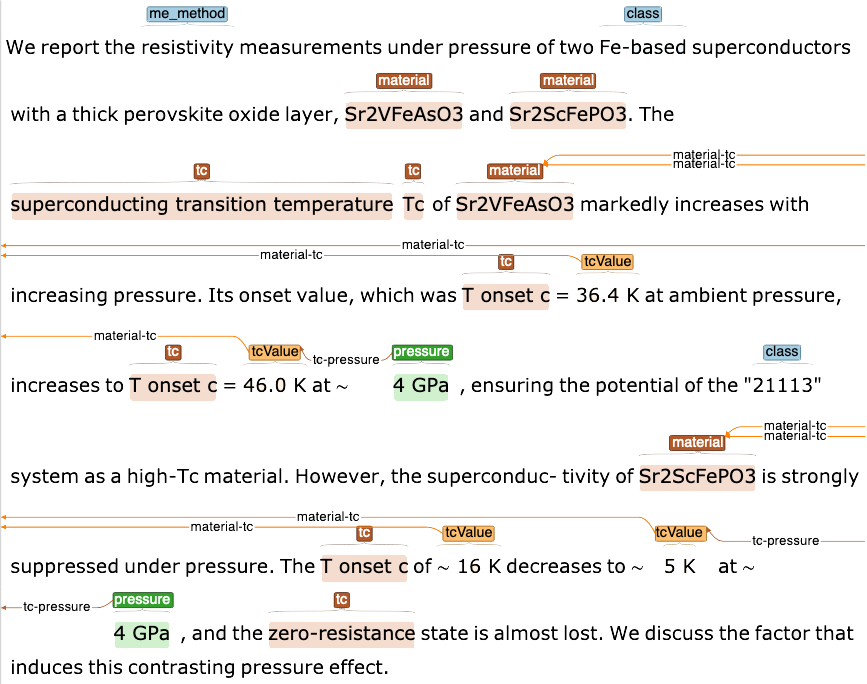
\includegraphics[width=\linewidth]{example-annotated-corpus-postprocess.png}
  \caption{Example of annotated corpus. The example is taken from~\cite{Kotegawa2009ContrastingPE}.}
  \label{fig:example-annotations-and-links}
\end{figure}

% \begin{figure}[htb]
%     \centering
%     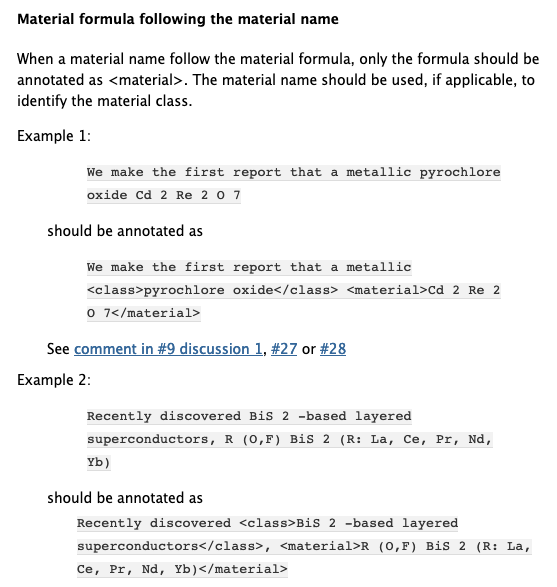
\includegraphics[width=0.9\linewidth]{example-guidelines-1b.png}
%     \caption{Example of a snippet of the guidelines. Each tag's description is further divided in several sub-sections discussing specific cases. They are supported with examples and discussions. We use a set of simple XML (eXtended Markup Language)\protect\footnote{\protect\url{https://www.w3.org/TR/xml11}} tags to describe the annotations.}
%     \label{fig:guidelines-example}
% \end{figure}

\begin{table}[ht]
    \centering
    \begin{tabular}{ | c | c| c| } 
    \hline
        \textbf{Iteration} \# & \textbf{IAA} & \textbf{IAA by label}  \\ [0.5ex] 
    \hline
        1  & 0.45
        &\begin{tabular}{  c | c  } 
            \texttt{<material>} & 0.45\\ 
            \texttt{<tc>} & 0.56\\
            \texttt{<tcValue>} & 0.50\\
            \texttt{<doping>} & 0.21\\
        \end{tabular}    
        \\ 
    \hline
        2 & 0.65
        &\begin{tabular}{  c |  c  } 
            \texttt{<material>} & 0.75\\ 
            \texttt{<tc>} & 0.85\\
            \texttt{<tcValue>} & 0.85\\
            \texttt{<doping>} & 0.39 \\
        \end{tabular}          
        \\ 
    \hline
        3 & 0.89
        & \begin{tabular}{  c | c  } 
            \texttt{<material>} & 0.89\\ 
            \texttt{<tc>} & 0.91\\
            \texttt{<tcValue>} & 0.88\\
            \texttt{<doping>} & 0.94\\
        \end{tabular}       
        \\ 
    \hline
    \end{tabular}
    \caption{Summary of the IAA for each annotation iterations.}
    \label{table:summary-preliminary-annotation}
\end{table}

% \begin{figure}[htb]
%     \centering
%     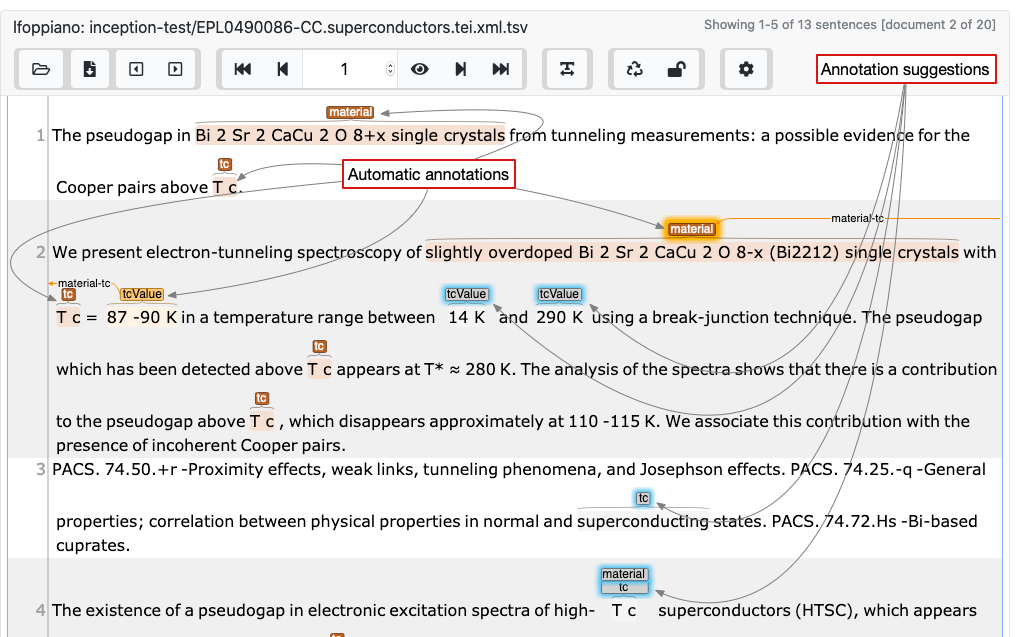
\includegraphics[width=\linewidth]{example-suggestions.png}
%     \captionof{figure}{Example of how automatic annotation and suggestions are appearing to the user. The automatic annotations are and look like normal annotations, while the suggestions are not applied by default unless the user click on them explicitly. The example is taken from~\cite{Mourachkine2000ThePI}.}
%     \label{fig:example-automatic-suggestions}
% \end{figure}

% \begin{figure}[htb]
%     \centering
%     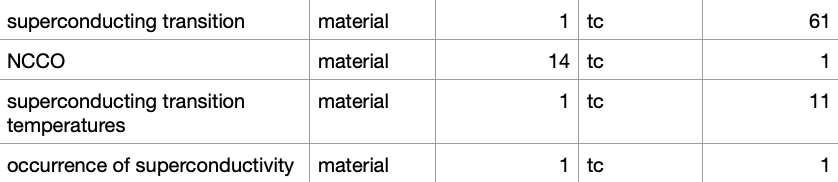
\includegraphics[width=\linewidth]{example-inconsistencies-clear-mistakes.png}
%     \captionof{figure}{Inconsistencies resulted from human mistakes.}
%     \label{fig:dataset-inconsistencies-clear}
% \end{figure}

\begin{table}[ht]
    \centering
    \begin{tabular}{ | c | c | c | c | c | } 
    \hline
        \textbf{Text} & \textbf{Label 1} & \textbf{\#} & \textbf{Label 2} & \textbf{\#}\\
    \hline
        \texttt{LiFeAs}         &   \texttt{<material>}   &    89   &   \texttt{<class>}  &   1   \\
        \texttt{Bi-2212}        &	\texttt{<material>}   &    34   &   \texttt{<class>}  &   1   \\
        \texttt{cobalt oxide}   &   \texttt{<material>}   &    89   &   \texttt{<class>}  &   1   \\
        \texttt{RE-123}         &	\texttt{<material>}   &    34   &   \texttt{<class>}  &   1   \\
    \hline
    \end{tabular}
    \caption{Inconsistencies resulted from human mistakes.}
    \label{table:dataset-inconsistencies-clear}
\end{table}

% \begin{figure}[htb]
%     \centering
%     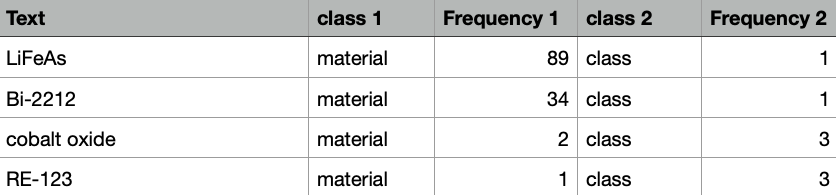
\includegraphics[width=\linewidth]{example-inconsistencies-doubious-mistakes.png}
%     \captionof{figure}{Inconsistencies resulted from material and class overlapping. }
%     \label{fig:dataset-inconsistencies-unclear}
% \end{figure}

\begin{table}[ht]
    \centering
    \begin{tabular}{ | c | c | c | c | c | } 
    \hline
        \textbf{Text} & \textbf{Label 1} & \textbf{\#} & \textbf{Label 2} & \textbf{\#}\\
    \hline
        \texttt{superconducting transition}     &   \texttt{<material>}   &    1   &   \texttt{<tc>}  &   61   \\
        \texttt{NCCO}    &	\texttt{<material>}   &    14   &   \texttt{<tc>}  &   1   \\
        \texttt{superconducting transition temperatures}     &   \texttt{<material>}   &    1   &   \texttt{<tc>}  &   11   \\
        \texttt{occurrence of superconductivity}    &	\texttt{<material>}   &    1   &   \texttt{<tc>}  &   1   \\
    \hline
    \end{tabular}
    \caption{Inconsistencies resulted from the overlapping of \texttt{<material>} and \texttt{<class>} labels.}
    \label{table:dataset-inconsistencies-unclear}
\end{table}

\begin{figure}[htb]
\centering
  \centering
  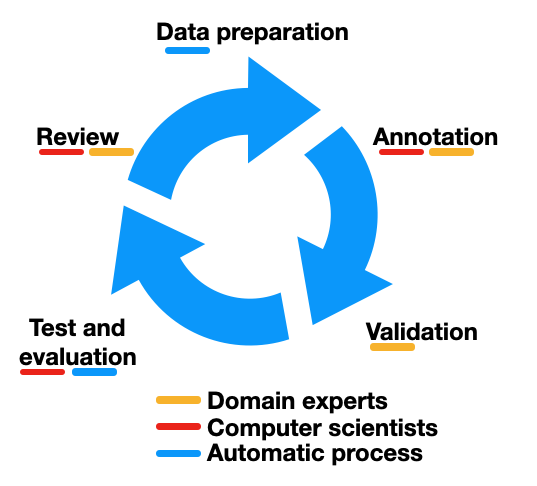
\includegraphics[width=0.5\linewidth]{workflow-schema}
  \caption{The annotation workflow. Different colours illustrate the involvement of each group at each step of the workflow.}
  \label{fig:schema-comparison-modified-workflow}
\end{figure}

\begin{figure}[htb]
    \centering
    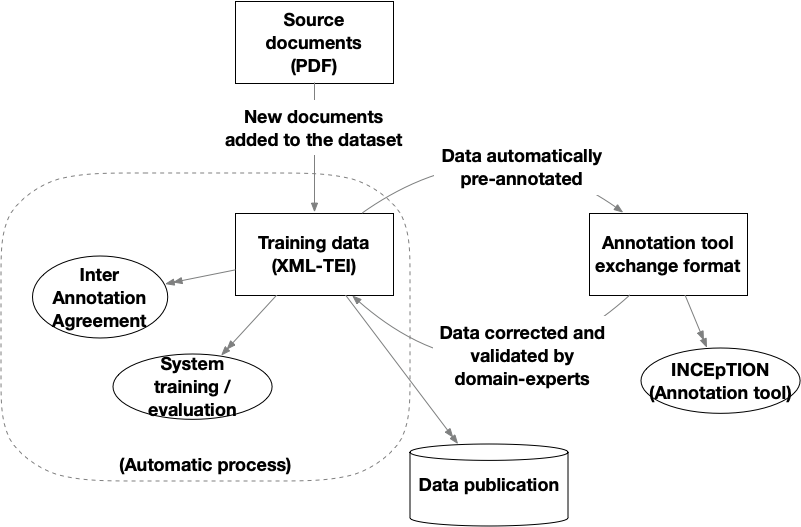
\includegraphics[width=\linewidth]{data-transformation.png}
    \captionof{figure}{Summary of the data transformation flows.}
    \label{fig:data-transformation}
\end{figure}

\begin{figure}[ht]
\begin{subfigure}{0.3\textwidth}
     \centering
    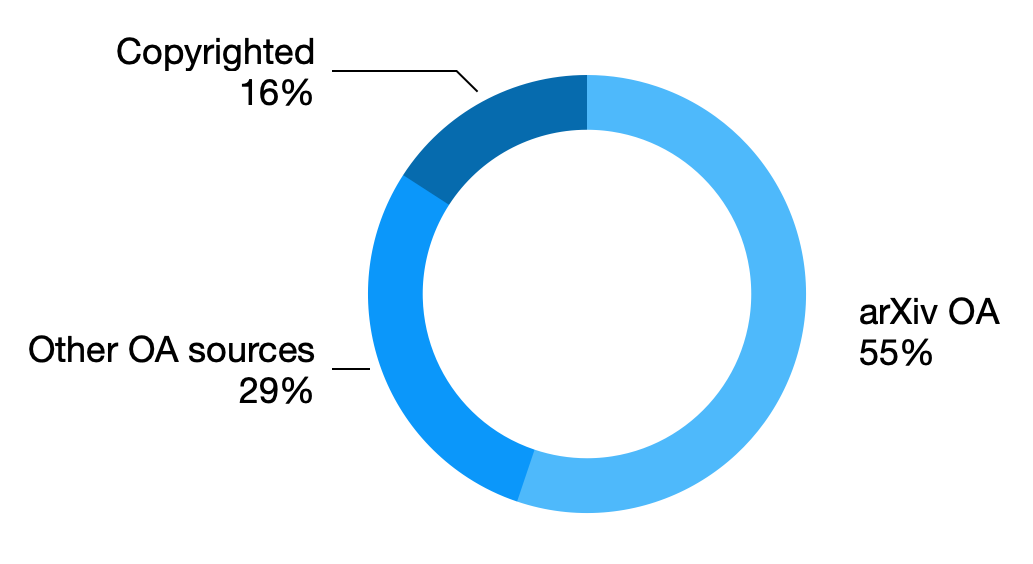
\includegraphics[width=\linewidth]{papers-by-sources.png}
    \captionof{figure}{Papers distribution by Licence (Open Access vs Copyrighted).}
    \label{fig:arxiv-rate}
\end{subfigure}
\begin{subfigure}{0.4\textwidth}
     \centering
    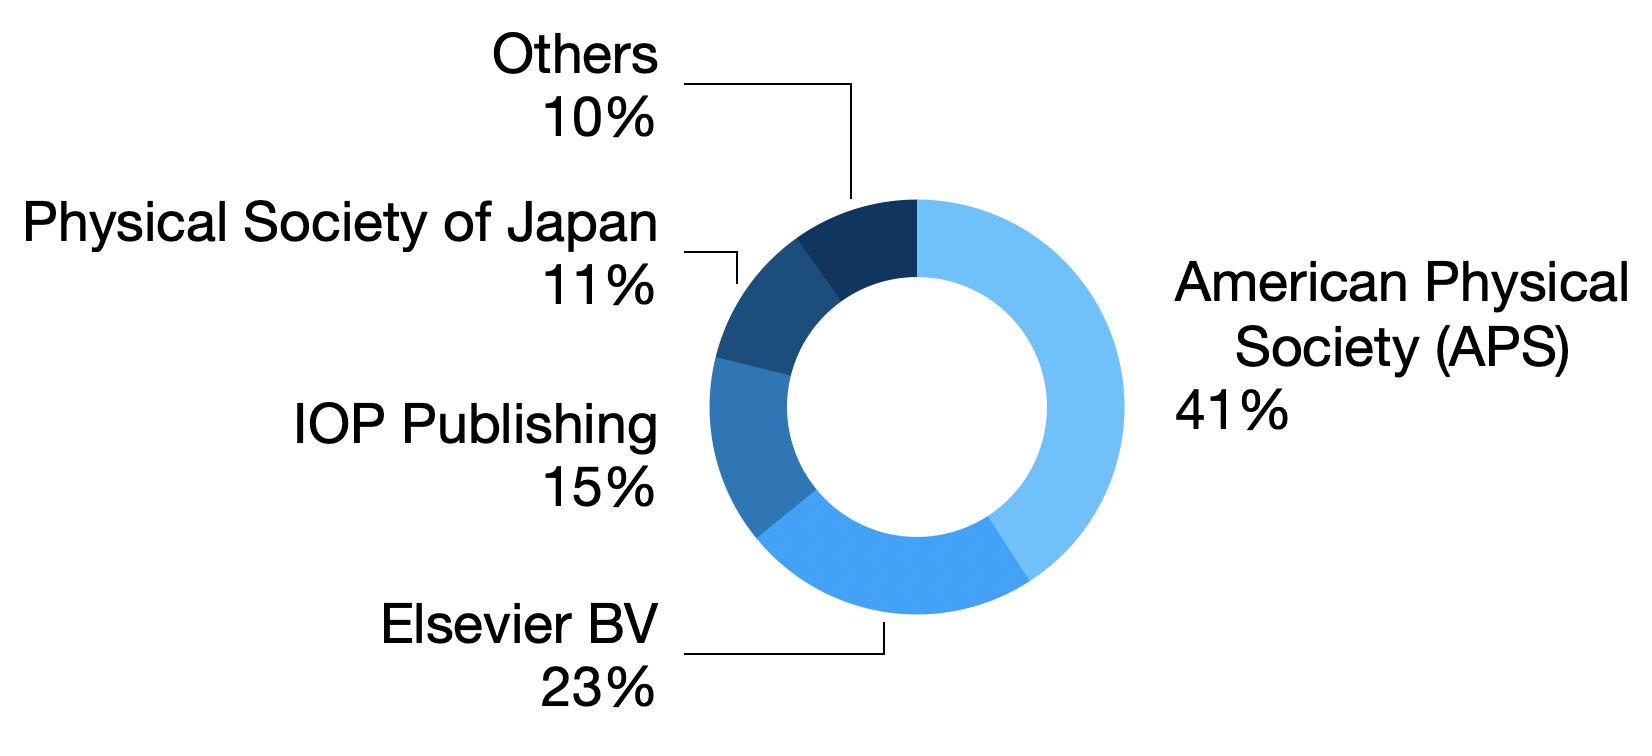
\includegraphics[width=\linewidth]{papers-by-publishers.png}
    \captionof{figure}{Distribution by publishers.}
    \label{fig:distribution-by-publisher}
\end{subfigure}
\begin{subfigure}{0.3\textwidth}
\centering
    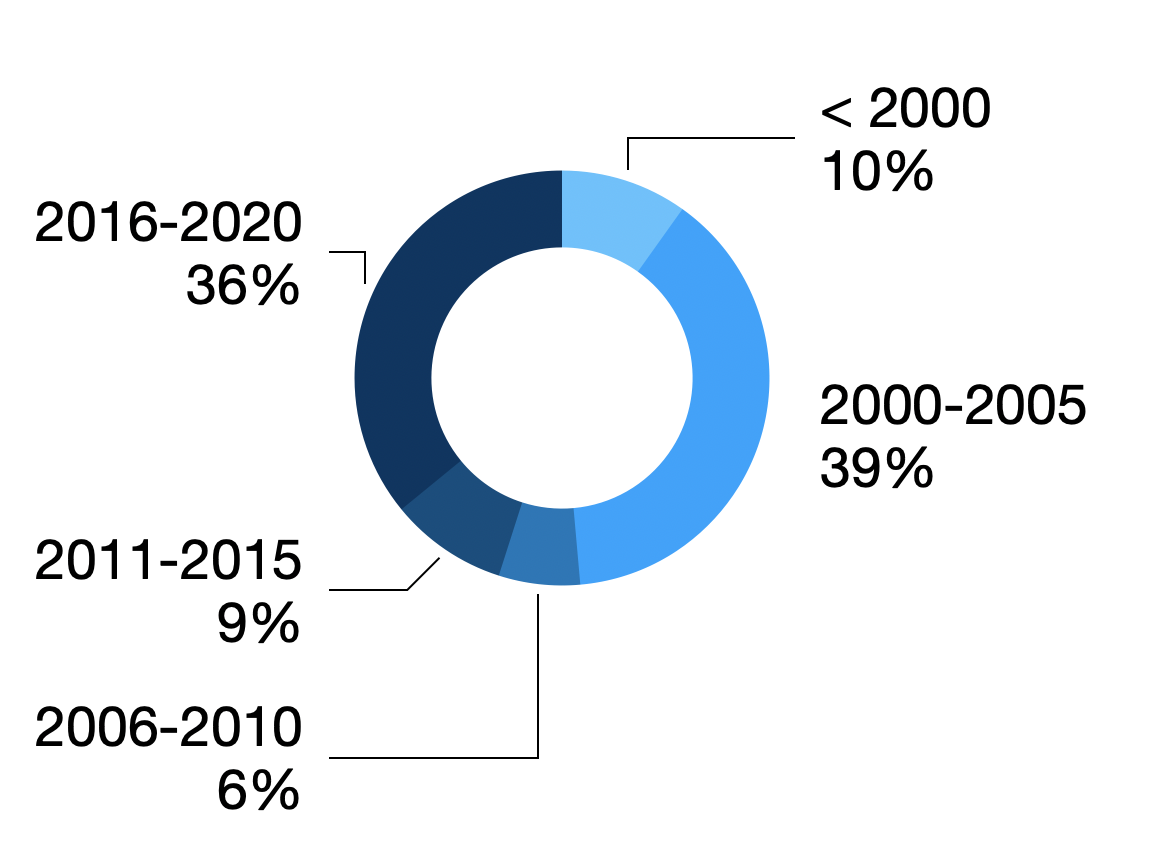
\includegraphics[width=\linewidth]{papers-by-years.png}
    \captionof{figure}{Distribution by years of publication.}
    \label{fig:distribution-by-year}
\end{subfigure}
\caption{Dataset distribution by years and publishers, automatically extracted from the PDF, and consolidated through a lookup to Crossref. }
\label{fig:dataset-distributions}
\end{figure}

\begin{figure}[htb]
    \centering
    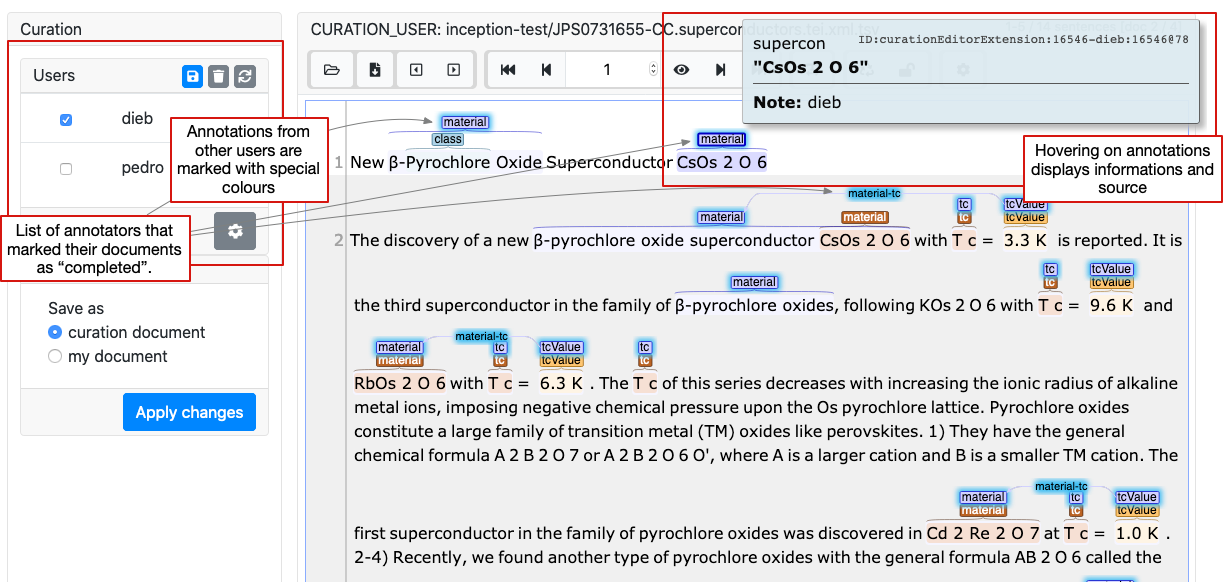
\includegraphics[width=\linewidth]{inception-curation-new.png}
    \captionof{figure}{INCEpTION curation interface. The example is taken from~\cite{Yonezawa2004NewO}.}
    \label{fig:inception-curation-interface}
\end{figure}

\begin{table}[ht]
    \centering
    \begin{tabular}{ |m{6em}  | m{4em} | m{6em} | m{7em} | m{6em} |} 
    \hline
        \multirow{2}{5em}{\textbf{Documents}} & \textbf{Files} & \textbf{Paragraphs} &	\textbf{Sentences} & \textbf{Tokens}\\
         & 114  &	2332 & 	14955 & 	4664\\
    \hline\hline
        \multirow{2}{5em}{\textbf{Entities}} & \textbf{Entities} &  \multicolumn{2}{|c|}{\textbf{Unique entities}} &  \textbf{ Labels} \\
        & 9966 &  \multicolumn{2}{|c|}{4000} &  6 \\
    \hline\hline
        \multirow{2}{5em}{\textbf{Links}} & \textbf{Links} & \multicolumn{2}{|c|}{\textbf{Links\textsubscript{ip}}} 
        & \textbf{Links\textsubscript{ep}}\\
        & 567  & \multicolumn{2}{|c|}{532}&	34	\\
    \hline
    \end{tabular}
    \caption{Statistical overview of the dataset. 
    Links\textsubscript{ip} (intra-paragraph) indicate the number of links within the same paragraph. Links\textsubscript{ep} (extra-paragraphs) indicate the number of links from different paragraphs.  }
    \label{table:summary-content}
\end{table}

% \begin{table}[hbt]
%     \centering
%     \begin{tabular}{ | c | c | c | c | c | c | c | c | } 
%     \cline{2-7}
%     \multicolumn{1}{c}{} & \multicolumn{3}{| c |}{\textbf{CRF}} & \multicolumn{3}{ c |}{\textbf{BidLSTM+CRF}} \\
%     \hline
%         \textbf{Label} & \textbf{Precision} & \textbf{Recall} & \textbf{F1} & \textbf{Precision} & \textbf{Recall} & \textbf{F1} \\
%     \hline
%         \texttt{<class>}        & 74.48 &   67.46 & 70.7  & 63.13 & 61.69 & 62.34  \\
%         \texttt{<material>}     & 77.95 &   75.38 & 76.63 & 74.48 & 76.69 & 75.56  \\
%         \texttt{<me\_method>}   & 63.78 &   59.5  & 61.47 & 66.53 & 74.69 & 70.34  \\
%         \texttt{<pressure>}     & 63.13 &   41.46 & 49.05 & 65.96 & 75.00 & 69.89  \\
%         \texttt{<tc>}           & 79.17 &   73.71 & 76.33 & 78.17 & 76.72 & 77.41  \\
%         \texttt{<tcValue>}      & 74.82 &   66.26 & 70.11 & 69.53 & 76.64 & 72.77  \\
%     \hline
%         \textbf{Micro avg}      & 75.86 & 71.2  & 73.45 & 72.61 & 74.84 & 73.71 \\
%         \textbf{Macro avg}      & 72.22 & 63.96  & 67.38 & 69.73 & 73.57 & 71.39 \\
%     \hline
%     \end{tabular}
%     \caption{Quantitative evaluation of a sequence labelling machine learning model.}
%     \label{table:evaluation-machine-learning}
% \end{table}

\begin{table}[ht]
    \centering
    \begin{tabular}{ | c | c | } 
    \hline
        \textbf{Label} & \textbf{Average}\\
    \hline
        \texttt{<material>}     &   0.946   \\
        \texttt{<me\_method>}   &	0.881   \\
        \texttt{<pressure>}     &	0.768   \\
        \texttt{<class>}        &	0.892   \\
        \texttt{<tcValue>}      &	0.856   \\
        \texttt{<tc>}           &	0.819   \\
    \hline
        \textbf{Micro average}        &	0.896	\\
    \hline
    \end{tabular}
    \caption{Average IAA between annotated and validated documents, over all the dataset [TODO: update table including batch 1, which is still due to be validated]}
    \label{table:average-iaa}
\end{table}

\begin{table}[ht]
    \centering
    \begin{tabular}{ | c | c | c | c | c | } 
    \hline
        \textbf{Label} & \textbf{Non-domain experts} & \textbf{Domain experts} & \textbf{Novices}\\
    \hline
        \texttt{<material>}     &   0.924   &   0.969   &   0.924   \\
        \texttt{<me\_method>}   &	0.807   &	0.890   &   0.901   \\
        \texttt{<pressure>}     &	0.72    &	0.836   &   0.746   \\
        \texttt{<class>}        &	0.802	&   0.990   &   0.899   \\
        \texttt{<tcValue>}      &	0.734	&   0.895   &   0.841   \\
        \texttt{<tc>}           &	0.771	&   0.874   &   0.830   \\
    \hline
        \textbf{All labels}        &	0.857	&   0.940   &   0.896   \\
    \hline
        \textbf{\# paragraphs}  &	423	    &   343     &   325     \\
    \hline
    \end{tabular}
    \caption{IAA calculated between annotations produced by non-domain experts, domain-experts and novices, and the final validated version. The data from non-domain experts and domain-experts has been sampled to provide comparable results. Annotation performed by one domain expert is validated by a different one. }
    \label{table:comparison-iaa-nde-de}
\end{table}

\end{document}
